\chapter{便 血}

血液从肛门排出,大便带血,或全为血便,色鲜红、暗红或柏油样,称为便血。

一般来说,便血较多提示下消化道(特别是结肠与直肠)出血。便血而伴有呕血提示上消化道出血。上消化道出血所排出的多是暗红色的血或黑便,呈柏油样,而下消化道出血所排出的多是较鲜红或鲜红色的血;两者均可有例外,下文将述及。

病史对两者的鉴别有重要意义。除消化道疾病外,便血也可能是全身性疾病所致出血的部分表现,例如白血病与淋巴瘤,患者往往伴有其他器官出血现象,以及全身性疾病的症状与体征。

口腔、鼻咽、喉、气管、支气管、肺等部位的出血,被吞咽后也由肛门排出。因此,诊断便血时须先排除上述疾病。此外还应注意与下列情况区别:

1.口服某些中草药、兽炭、铁剂、铋剂时,大便可呈暗褐色或黑色,但大便隐血试验呈阴性。

2.食用过多的肉类、猪肝、动物血之后大便可变暗褐色,大便隐血试验呈阳性,但素食后即转呈阴性。免疫法大便隐血试验则呈阴性。

3.口服酚酞制剂,大便有时呈鲜红色,不注意时易误认为大量便血。

便血的颜色取决于消化道出血的部位、出血量与血液在肠道停留时间。上消化道出血如伴有肠蠕动加速时,则可排出较鲜红的大便而不呈黑便。小肠出血时,如血液在肠内停留时间较长,可呈柏油样大便;当出血量多,排出较快时则呈暗红色,甚至鲜红色稀便或紫红色血块,排出的血块有时可见空肠黏膜环纹印迹。结肠和直肠出血时,由于血液停留于肠内时间较短,往往排出较新鲜血液。上位结肠出血时,血与大便常混杂;乙状结肠和直肠出血时,常有新鲜血液附着于成形大便的表面。

少量便血多来源于直肠、乙状结肠或降结肠疾病,如痔、溃疡、息肉与癌,也见于肠套叠等;中等量便血多见于肠系膜及门静脉血栓形成;大量便血应考虑来自上消化道或急性出血性坏死性肠炎、肠伤寒等疾病,此外有时也见于回肠远端憩室溃疡、结肠憩室病、缺血性结肠炎等。

血在大便后滴下,与粪便不相混杂者多见于内痔、肛裂,也可见于直肠息肉与直肠癌。血与粪便相混杂,伴有黏液者,应注意结肠癌、结肠息肉病、溃疡性结肠炎。

粪便呈脓血样,或血便伴有黏液及脓液,须考虑痢疾、结肠血吸虫病、溃疡性结肠炎、结肠结核等。

便血伴有剧烈腹痛,甚至出现休克现象者,应注意肠系膜血管阻塞、出血性坏死性肠炎、缺血性结肠炎、肠套叠等的可能。

便血伴有腹部肿块者,须想到结肠癌、肠套叠与放线菌病等。

便血伴有皮肤或其他器官出血现象者,多见于血液病、急性感染性疾病、重症肝脏病、尿毒症、维生素C缺乏症等。

详细的病史与体检(特别注意全身性出血表现、腹部肿块和必要的妇科检查),对便血病因的诊断与鉴别诊断有重要意义。直肠指检对原因未明的便血是必要的,大多数的直肠癌可被触及。大便镜检可发现结肠炎的病理成分、寄生虫卵与某些寄生虫;大便孵化法可找到血吸虫毛蚴;大便培养可发现致病菌。直肠乙状结肠镜检查不但能直接窥视直肠、乙状结肠病变情况,并可取出内容物做镜检或做活体组织检查。结肠镜能观察到全段结肠及末段回肠的病变。钡餐胃肠透视与钡剂灌肠造影检查,可在出血停止后一段时间内施行,对胃肠道溃疡、憩室、息肉、肿瘤等诊断均有帮助。

原因未明的便血也非少见,须注意常规检查未能发现或较难发现的疾病,如小肠憩室、血管瘤,如条件许可,有指征时可作一些特殊的检查,如胶囊内镜、单/双气囊小肠镜、CT小肠成像(CTE)或MR小肠成像(MRE)、放射性核素铬示踪红细胞显像,选择性动脉造影等协助诊断。

先天性血管畸形所致下消化道出血往往难于诊断。罹患部位一般多在盲肠与升结肠,病变在黏膜下层,X线钡剂灌肠造影与结肠镜检查、甚至剖腹探查也常无发现。如在出血期间作选择性肠系膜上、下动脉造影,或(及)作放射性核素示踪红细胞显像,常有助于确定诊断。

门脉高压症引起的静脉曲张破裂出血,一般位于食管下段或胃底静脉,偶尔也有回肠末段、结肠、直肠与乙状结肠交接处或直肠的静脉曲张破裂出血。如门脉高压症患者有便血而无食管或胃底静脉曲张破裂,则须考虑上述罕见部位的静脉曲张出血。这些罕见的静脉曲张破裂出血,在手术探查或病理解剖时,甚难发现有扩张的静脉分流存在,除非已有血栓形成。临床上,这些病例只有在出血后短期内作结肠镜检查,或在出血时作肠系膜上、下动脉造影,或(及)作放射性核素示踪红细胞显像检查,才能确定出血灶的部位。

小肠出血的诊断近年有重大的发展。小肠出血的原因很多,有溃疡、肿瘤、憩室、血管异常等。

近几年发展起来的小肠检查技术使小肠出血病灶的发现取得了重大进展。这些技术包括胶囊内镜(CE)、单/双气囊小肠镜(SBE/DBE)、血管造影、小肠CTE/MRE等。CE和(SBE/
DBE)是诊断小肠出血的有效手段,对CE和DBE的对比研究中发现它们对不明原因的消化道出血(OGIB)诊断价值相似,病因诊断率为81\%~91\%。也有人认为DBE在OGIB的确诊率方面要优于CE,DBE可以发现CE不能发现的微小病灶。通常CE可作为常规检查阴性而经济条件优越患者首选的筛查性检查,联合CE和DBE有助于提高OGIB确诊率。数字减影血管造影(DSA)对血管病变所致小肠出血,特别对一些出血量大、以血管病变为主需选择介入治疗的病例,不失为一种有价值的检查治疗手段,小肠出血速度大于0.5ml/min时,DSA的诊断准确率为12\%~69\%,差异可能与出血速度、病变性质、造影时机选择及操作人员技术等因素有关。近年多层螺旋CT小肠造影技术(MSCTE)及MRE三维重建的强大后处理功能对小肠出血病因的诊断具有极高的价值,显示小肠整体形态结构可发现肠道肿瘤、炎症及憩室等病变,还可清楚显示肿瘤的大小、形态、性质、内部血供情况以及结构层次,明确有无浸润、转移情况,有助于肿瘤分期,同时还可对内脏肠道小血管进行显像,发现血管畸形、出血血管,可清楚显示活动性出血所在血管以及与邻近血管的关系和情况。

国外报道,小肠出血的病因以血管发育异常最常见,多见于老年人;其次是小肠肿瘤,包括平滑肌瘤、类癌、淋巴瘤以及腺癌等,而溃疡和糜烂(包括药物性和克罗恩病)、憩室等相对较少。中山大学附属第一医院报道小肠出血前三位的病因是小肠良性溃疡(包括克罗恩病)、肿瘤、血管畸形,其次是梅克尔憩室、寄生虫感染、憩室炎、小肠结核、Behet病、蓝色象皮疮样痣综合征等。

下消化道出血的病因相当复杂,各家报道各病种的发生率差别较大。如国内外科报道的一组2077例病例,恶性肿瘤占最多数(1110例)、息肉次之(452例)、炎症又次之(295例)、良性肿瘤最少(4例);恶性肿瘤又以直肠癌最多、结肠癌次之。另朱琪麟等对1542例下消化道出血患者肠镜检查结果进行分析,结果显示下消化道出血的常见病因依次为肠息肉(31.8\%)、结直肠癌(18.4\%)、肛门肛周病变(17.7\%)、慢性结肠炎(14.8\%)、炎症性肠病(9.6\%)。

便血的病因按表\ref{tab22-1}的分类顺序讨论如下:

\begin{table}[htbp]
\centering
\caption{便血疾病的分类}
\label{tab22-1}
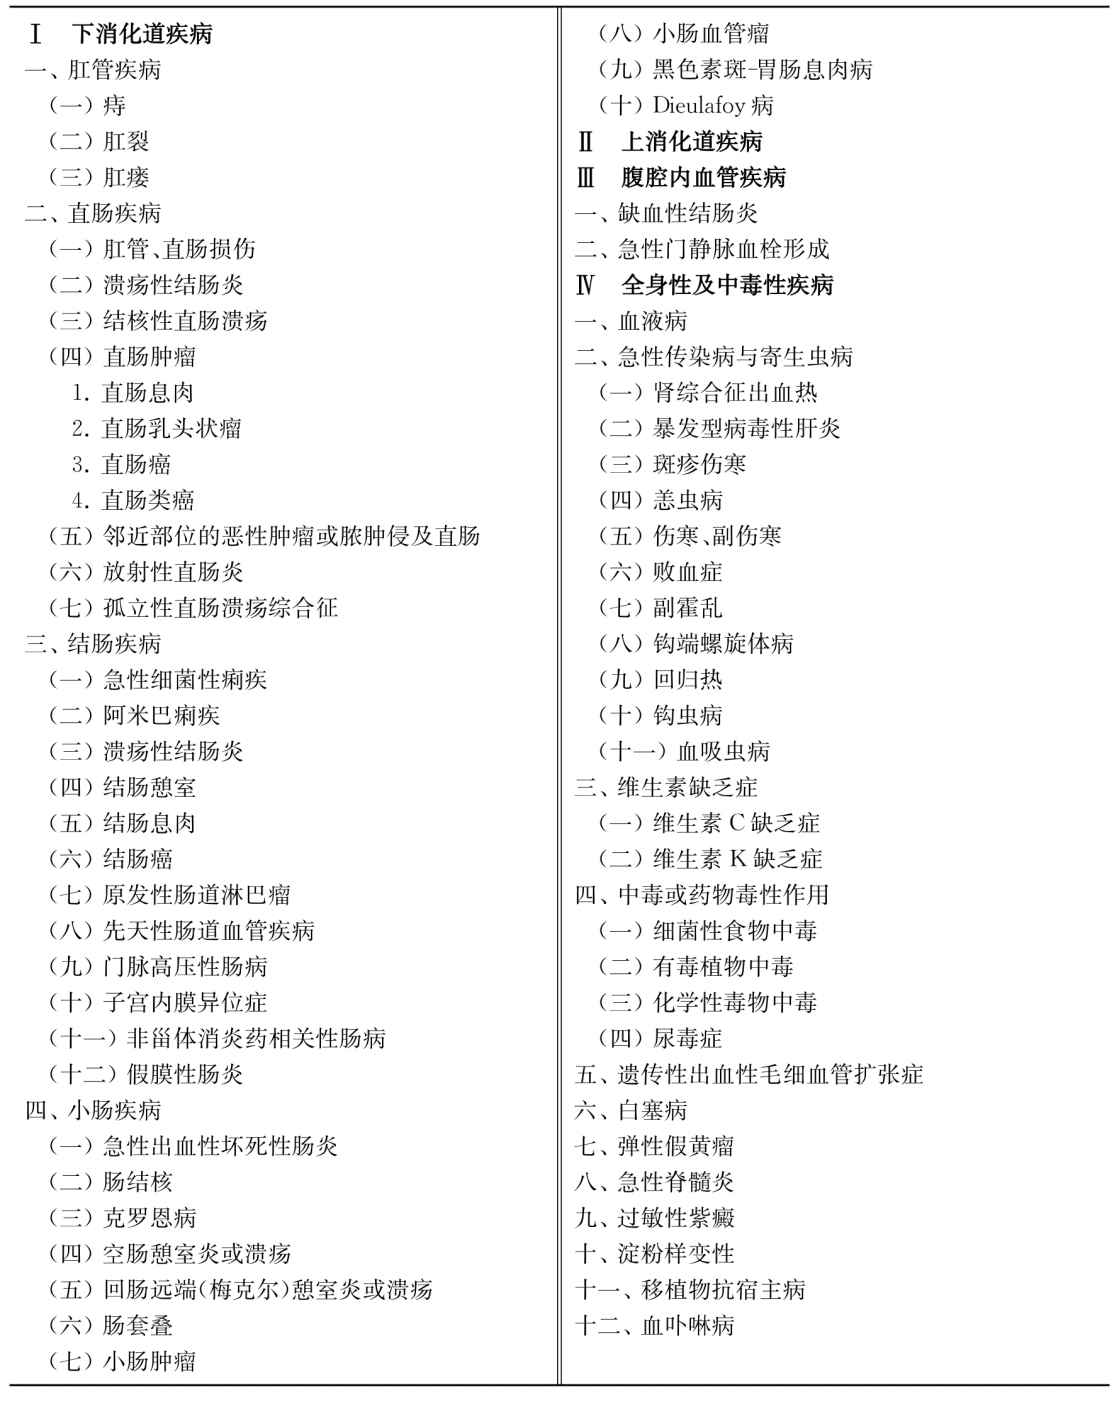
\includegraphics[width=5.91667in,height=7.41667in]{./images/Image00123.jpg}
\end{table}

\protect\hypertarget{text00174.html}{}{}

\section{69 下消化道疾病}

\subsection{69.1 肛管疾病}

\subsubsection{一、痔}

内痔与混合痔,特别是第Ⅰ、Ⅱ度内痔多以便血为其主要症状。便血一般发生于排便时,呈喷射状流出,或在便后滴出鲜血,血与粪便不相混。出血量多少不等,一般为数毫升至十几毫升。反复出血可导致严重贫血。便血是由于排便时腹内压增高,致痔内静脉丛血压随之升高,加上硬粪的直接擦损,使痔破裂所致。患者可伴有肛门异物感或肛门疼痛。肛门视诊可见各类型外痔,直肠指检可触到内痔。脱出肛外的内痔及混合痔,可在肛门外观察到,呈圆形突起的暗红色小肿物;位于肛门内的痔核,嘱患者做用力排便动作时,也可脱出而看到。肛管镜检查时,内痔在肛管直肠环平面以下,呈圆形,暗红色的痔块突入镜内。

根据上述的临床表现与检查一般较易对痔进行诊断。但必须指出,临床上也可将具有便血症状的肛管直肠疾病,如有蒂的直肠息肉、直肠癌误诊为内痔。另一方面,有些便血的疾病如直肠癌,同时伴有痔时,如不细致检查,发现痔后即满足于诊断,以致延误癌的诊断与治疗者也有之。因此确定痔的诊断时,须细致排除其他肛管直肠疾病。

\subsubsection{二、肛 裂}

肛裂发生于肛管下缘,初起时大都为一线状裂缝,以后继发感染、扩大而形成小溃疡,排便时引起剧烈的疼痛。肛裂是小儿便血症最常见的原因。儿童可因蛲虫感染引起肛周瘙痒、抓破、感染而形成。90\%以上的肛裂位于肛管后中线,痔核间沟平面或以上。常为单发。

肛裂的典型症状是排便时及排便后不同程度的周期性疼痛,伴有便血,与痔的临床表现不同。便血量少,色鲜红,呈丝状覆盖于粪便的表面,常在排便时或紧接在便后出现。肛门视诊可见袋状皮垂(前哨痔),轻轻向两侧翻开肛门皮肤或同时嘱患者用力使肛管外翻,常可发现溃疡的下端或全部。溃疡呈卵圆形、边缘齐整、底呈红色,慢性者裂缘不整、底深、呈灰白色。

\subsubsection{三、肛 瘘}

肛瘘常有脓性分泌物流出,但很少为血性。本病最常继发于肛管直肠周围脓肿;少数为结核性,常继发于肺结核或肠结核。体检在肛门附近、会阴部或骶尾部等处可见肛瘘外口。挤压其周围组织即有少许脓液从瘘口流出。直肠指检及肛窥器检查可发现瘘管内口。如为直瘘,由瘘外口插入探针可经瘘管通到内口,手指在肛管直肠内可触及探针前端。

\protect\hypertarget{text00175.html}{}{}

\subsection{69.2 直肠疾病}

\subsubsection{一、肛管、直肠损伤}

便秘时,偶尔坚硬的粪块擦破肛管直肠黏膜,以致发生小量出血,色鲜红,常覆盖于粪便的表面,有时伴少量黏液。损伤一般愈合很快,也不再出血。

作直肠乙状结肠镜检查,如操作不过细,可损伤肛管直肠黏膜,而引起小量出血,但不久自止。在采取活体组织后,有时出血量颇多。

\subsubsection{二、溃疡性直肠炎}

上海报道一组溃疡性结肠炎486例,其中溃疡性直肠炎占142例(28.8\%)。本病患者常以解便次数增加、伴轻度下腹痛为主诉,有的有黏液便或黏液血便,甚至小量便血。个别还有便秘。但其最具特征性的症状是里急后重。内镜所见与溃疡性结肠炎基本一致,可有黏膜充血、水肿、糜烂、脆易出血。很多小浅溃疡位于弥漫性炎症黏膜的背景中。诊断与鉴别诊断主要依靠肠镜检查。病程迁延,可历经数年。长期随访,一部分病例发展为直肠乙状结肠炎。

\subsubsection{三、结核性直肠溃疡}

严重而广泛的肠结核可向下蔓延累及直肠形成溃疡,可发生脓血样大便。患者常伴有腹泻便秘交替、下腹疼痛、里急后重、食欲不振、体重减轻等症状。直肠镜检查可发现与癌性溃疡、性病性肉芽肿溃疡或慢性结肠炎相似的病变。此病的溃疡常侵及肛门黏膜及附近皮肤,溃疡分泌物可找到结核菌,患者多有肺结核病史,可与以上疾病相区别。X线钡餐、钡剂灌肠、病灶活体组织检查等也可协助诊断。

\subsubsection{四、直肠肿瘤}

\paragraph{(一)直肠息肉}

结肠及直肠息肉是常见的良性肿瘤,临床上大多发生于直肠与结肠后壁,文献报道结肠及直肠息肉位于乙状结肠以上者占20\%左右。结肠及直肠息肉在成年人及儿童皆不少见,大多数是单个腺瘤,少数为多个。小的息肉可无症状。有症状的息肉多较大,或为多发性,其主要症状是便血,多为间歇性,色鲜红,一般量不多,不与粪便相混。有些患者表现为慢性脓血样腹泻,易与痢疾、慢性结肠炎相混淆,但细心观察患者的大便,往往可见成形的粪便,一侧有凹陷压迹。

国内文献曾报道在一些儿童中发现直肠息肉。凡有大便带血而大便次数与性质基本正常的儿童患者,应首先考虑直肠息肉的可能。息肉附着于直肠壁的基部,或为扁平状,或为蒂状。如便后有红色分叶状小肿物脱出于肛门外,便后不久又缩回肛内者,则很可能为蒂状息肉。直肠指检可触到有蒂的、圆形或卵圆形、可移动的、表面光滑的、软质的小肿物,但一些直肠息肉不易触到,故直肠乙状结肠镜检查是重要的诊断手段。结肠气钡双重造影X线检查或结肠镜检查有助于多发性结肠息肉(结肠息肉病)的诊断。

直肠的多发性息肉常为结肠息肉病(参见第69.3节)的部分表现。扁平的直肠息肉与癌变有一定的关系,一般认为是一种癌前期病变。

\paragraph{(二)直肠乳头状瘤}

直肠乳头状瘤少见,国外文献报道最小发病年龄为15岁,最大为89岁,平均年龄约为60岁,80\%以上发生于直肠与乙状结肠。其常见症状是便血,但严重出血者少见,故重度贫血不常见。此瘤在直肠乙状结肠镜下呈基底宽的息肉样肿物,浅红色至深红色,状如海绵,浸浴于透明的蛋清黏液中,大小为2~15cm。钡剂灌肠X线检查可能表现为类似结肠癌的显影。此瘤的恶变倾向甚大。

\paragraph{(三)直肠癌}

直肠癌是常见的恶性肿瘤,约70\%发生于直肠上1/3和直肠与乙状结肠交界处附近。多见于30~70岁中、老年人,国内报道男多于女。直肠癌在华南地区占消化道癌的首位。有些临床医生认为便血是直肠癌的第一个症状,但此时癌往往已发展至相当程度。便血初期只有少量血液附着于粪便表面,以后随病情发展,便血量较多。患者逐渐出现轻度腹泻、里急后重、体重减轻、贫血等症状。粪便常混有脓液或黏液,有特殊腥臭味,与痔、慢性结肠炎、细菌性痢疾的便血不同;大便镜检无溶组织阿米巴滋养体,可与阿米巴性痢疾相区别。直肠癌入院时误诊最多者为痢疾。

凡30岁以上的(甚至较年轻的)患者有未明原因的便血或大便带脓血,须注意直肠癌而进行必要的检查;如有进行性贫血、消瘦,则往往是直肠癌的后期现象。此时直肠指检大多数在肠壁上可触到形状不整齐、质硬、呈结节状的肿块,或可触及向外翻的、边缘隆起的硬性溃疡,检查指套往往染有血液和黏液。如直肠指检阴性,须作直肠乙状结肠镜检查,不但可直接观察到肿块或癌性溃疡,并可在直视下作活检,后者是最可靠的直接诊断方法。如直肠发生癌性狭窄,直肠乙状结肠镜不能通过,则钡剂灌肠可了解癌以上的肠段情况。

\paragraph{(四)直肠类癌}

国内报告一组36例消化道类癌中,直肠类癌占16例,阑尾类癌占10例。患者多无症状;部分患者则以便血、便秘、腹泻与直肠部疼痛为首发症状。除少数患者指检可触及小肿块外,体检一般无阳性体征发现。直肠镜检查可见类癌呈黄灰色乃至浅棕红色,球状或扁豆状,表面一般无溃疡。国内报告的36例中,良性者占61.2\%,恶性者占38.8\%。

\subsubsection{五、邻近部位的恶性肿瘤或脓肿侵入直肠}

直肠邻近脏器的癌(如子宫颈癌)、盆腔脓肿等侵入直肠时可产生便血。患者有原发病的症状与体征。

\subsubsection{六、放射性直肠炎}

放射性直肠炎属后期放射反应。用镭或深部X线作盆腔内放射治疗子宫颈癌,可伤及直肠,可在治疗后数周至数年出现里急后重和血性腹泻的症状,病理解剖检查发现肠管增厚与僵硬、溃疡形成、狭窄、血管损害、浸润及炎性病变等,须注意与其他疾病所致的便血相区别。

\subsubsection{七、孤立性直肠溃疡综合征}

孤立性直肠溃疡综合征(SRUS)是一种少见的非特异性良性疾病,病因尚不明确。文献报道该病可能与直肠脱垂和直肠内套叠、骨盆底肌肉的矛盾性收缩、创伤包括手指或器械插入直肠及肛交等造成的损伤、放射治疗和麦角胺栓剂的使用等有关。临床表现以血便、黏液血便、排便困难为主,是一种功能障碍性疾病,常见于30岁的男性和40岁的女性,也见于儿童和老年人。便血量可为新鲜少量,也可发生大出血需要输血治疗。内镜下表现也各不相同,从单纯的黏膜充血到小的或大的溃疡再到广基的、不同大小和数量的息肉。典型的SRUS是周围黏膜充血的表浅溃疡。40\%的患者有溃疡,其中20\%是孤立性溃疡,其余的表现为黏膜充血、息肉,且其大小和形状各不相同。

\protect\hypertarget{text00176.html}{}{}

\subsection{69.3 结肠疾病}

\subsubsection{一、急性细菌性痢疾}

急性细菌性痢疾的大便呈脓血样,量少,次数频繁,常伴有腹痛、里急后重及毒血症症状。

\subsubsection{二、阿米巴痢疾}

阿米巴痢疾的大便呈暗红酱色,黏液较多,有恶臭味。部分患者以便血为主要表现。里急后重较细菌性痢疾为轻,右下腹常有压痛。

\subsubsection{三、溃疡性结肠炎}

主要表现为腹痛、腹泻、黏液血便。病情迁延,症状可持续或间歇出现。确诊有赖于结肠镜检查。

\subsubsection{四、结肠憩室与憩室炎}

结肠憩室是结肠壁上向外突出的袋状物,最多位于乙状结肠。患者多年龄超过40岁,体格肥胖,常坐位工作,有便秘习惯。憩室的形成一般认为是肠腔内压力增高和肠壁薄弱所致。无并发症的憩室无症状。如憩室发炎,则出现腹痛、发热、白细胞增多、局限性腹部压痛等症状。由于乙状结肠为好发部位,局部症状也多位于左下腹部。约20\%病例出现轻度与间歇性便血。诊断须于炎症消退后作钡剂灌肠X线造影检查。如结肠憩室为多发性,则称为结肠憩室病。

国外文献曾报告约6\%~10\%结肠憩室病发生大出血。中等量或大量出血者不少缺乏憩室炎的症状,而突然自发出血,失血量有达1000ml以上。

\subsubsection{五、结肠息肉}

结肠息肉是指高出于黏膜突向肠腔的赘生物。病理学上包括肿瘤性息肉(腺瘤)、错构瘤性息肉(幼年性息肉、Peutz-Jeghers息肉等)、增生性和炎症性息肉。国内一组796例大肠息肉病理分析显示,腺瘤性占43.8\%,炎症性占42.1\%,其余为增生性、幼年性。临床表现为便血(40\%)、腹泻(16.7\%)、腹痛(15.1\%)、黏液便(10.1\%)。部分患者无症状,肠镜检查时才发现。

结肠息肉病少见,患者大多为青年人,儿童次之。病变为家族性,可有大出血。大体解剖所见为结肠与直肠黏膜上满布大小不一的腺瘤样和小乳头样息肉。其临床特点是腹泻、便带鲜血和黏液,可因反复出血而引起贫血。结肠镜检查与钡剂灌肠X线检查,均有助于明确诊断。

结肠息肉病具有遗传性,且有高度恶性变的倾向。幼年性息肉病为常染色体显性遗传性疾病。其特点是多发性胃肠道幼年性息肉,主要累及结直肠。幼年性息肉病患者结直肠癌的几率为30\%~40\%,患者必须结肠镜随访观察。结肠息肉病伴有骨瘤病、纤维瘤病与囊肿者称为Gardner综合征;结肠息肉病伴有脑瘤者称为Turcot综合征。

\subsubsection{六、结肠癌}

结肠癌的临床表现因病变的部位不同而异。一般认为左侧结肠癌以亚急性或慢性肠梗阻为主要表现,晚期常因癌溃破而出现鲜红色便血,或伴有黏液与脓液;右侧结肠癌则以进行性贫血、腹块、不规则发热、腹泻为主要症状,大便除潜血试验阳性外,甚少出现鲜红色便血。但有不少例外。国内报告盲肠腺癌病例1/5有便血。钡剂灌肠X线检查是最常用的诊断方法。乙状结肠镜长度有限,只能观察到直肠与乙状结肠。全肠镜能观察到深部结肠病变,直到回盲部,并在直视下作活组织检查。结肠癌脱落细胞检查的具体操作要求高,阳性率仅为2/3病例,阴性不能除外癌,故应用有所限制。

大肠癌的发病既有遗传因素,又有环境因素。明确高危因素,对高危人群进行筛查有重要意义。病例研究表明大肠癌的高危因素有肠息肉史、慢性腹泻、慢性便秘、黏液血便、精神刺激史、饮水不洁史、阑尾手术史和家族肿瘤史。对年龄超过40岁有高危因素者可行免疫法大便隐血试验,必要时行大肠镜筛检,对大肠癌的早期诊断有意义。值得注意的是,在早期大肠癌中,约一半病例大便隐血试验呈阴性反应。

\subsubsection{七、原发性肠道淋巴瘤}

原发于胃肠道的淋巴瘤大多起源于B细胞,肠道T细胞淋巴瘤相对少见,T细胞淋巴瘤临床症状无特异性,多为腹痛、腹泻、发热及体重下降,病程中常常发生消化道大出血及急性肠穿孔等并发症,预后极差。肠镜下表现为多灶性溃疡性者常误诊为炎症性肠病,本病诊断主要依靠病理及免疫组化,但病理常常难以诊断,需多次活检或做大块黏膜切除病理以提高诊断率。

\subsubsection{八、先天性肠道血管疾病}

先天性肠道血管疾病包括肠道血管发育不良、血管瘤、遗传性毛细血管扩张等,其中血管扩张症、动静脉畸形占老年下消化道出血的50\%。血管畸形的病因未明,该病可能是老年人反复发生下消化道出血的病因之一,诊断依靠肠系膜血管造影和结肠镜。结肠镜下血管畸形分为局限型、蛛痣型、弥漫型及血管瘤样型,病变累及的部位以单发为主,病灶一般不大,好发部位以右半结肠最为常见。

\subsubsection{九、门脉高压性肠病}

门脉高压可导致门-体侧支循环的开放,临床上以食管-胃的侧支通路为最多见,常引起出血。门脉高压所致门-体侧支循环还可发生于以下诸多部位:十二指肠、空肠、回肠、回盲部、升结肠、降结肠、乙状结肠直肠交界处及直肠。门脉高压患者结肠镜下见静脉曲张,而组织炎症不明显,并能排除其他疾病所致的病变则可考虑为门脉高压性肠病。

\subsubsection{十、子宫内膜异位症}

子宫内膜异位症的发病特点为育龄妇女与月经有关的周期性便血、腹痛,内镜活检可确诊。多见于直肠、乙状结肠受累,约占75\%~90\%,小肠偶有发病。

\subsubsection{十一、非甾体消炎药相关性肠病}

随着非甾体消炎药(NSAIDs)的广泛应用,胃肠道副作用日渐突出,NSAIDs药物不仅可引起胃十二指肠溃疡的损伤,还可出现肠道损伤,尤其是老年人和需要长期服用的患者。NSAIDs相关性肠病下消化道出血量较大,使用质子泵抑制剂(PPI)治疗效果欠佳,结肠镜检查常可在回肠末端、结肠发现有节段性浅溃疡,黏膜红斑、糜烂及出血等病灶,有助于诊断。NSAIDs相关性下消化道出血多伴有上消化道出血和(或)上消化道溃疡,但较少出现肠腔狭窄、肠穿孔等并发症。

\subsubsection{十二、假膜性肠炎}

假膜性肠炎是一种医源性并发症,常出现在抗生素治疗之后,主要是发生于结肠的急性黏膜坏死炎症。腹泻是其最主要的症状,腹痛及毒血症表现亦见,肉眼血便少见。难辨梭状芽胞杆菌及其毒素为本致病因素。文献报道1例假膜性肠炎以反复、大量下消化道出血为突出表现,临床上极为少见。如应用大量广谱抗生素治疗出现无法解释的下消化道出血,应想到假膜性肠炎,假膜性肠炎致下消化道出血原因,考虑为病变严重侵及肠壁小血管所致。

\protect\hypertarget{text00177.html}{}{}

\subsection{69.4 小肠疾病}

\subsubsection{一、急性出血性坏死性肠炎}

国内报道颇多,其发病原因尚未完全明了,有认为是过敏性炎性病变,也有认为与肠道细菌感染有关。其出现为散发性,可在一个地区的不同居民点先后发生多例,与肠道细菌感染不相同。本病多发生于小儿与青少年。男性发病率高于女性。病变最常侵犯小肠,特别是空肠上段,而结肠有时也可累及。主要的病理改变是肠黏膜充血、水肿、出血与坏死,可侵及肌层与浆膜层,病灶呈节段性,也可为散在性或广泛性,其间可有正常肠段存在,并伴有肠系膜及所属淋巴结炎症性肿胀。

该病有四个主要临床特征:突发性急性腹痛、腹泻、便血和毒血症。患者发病前多有不洁饮食或暴饮暴食史,也可无任何诱因而突然发作。腹痛多位于左上腹或左中腹部,也可位于脐部甚或全腹。疼痛性质可为持续性隐痛或剧痛,经过数小时或十几小时后逐渐缓解,但不久又再发作,可呈阵发性绞痛。常伴有恶心、呕吐。进食小量食物也可加剧疼痛或引起绞痛发作。腹泻常随腹痛同时发生,早期为黄色水样,有的无明显血便。患者发病后1~2天内即出现衰弱无力、面色苍白、寒战、发热、不同程度的脱水、白细胞增多与核左移、中毒性颗粒出现等毒血症表现。腹部检查可发现中等度鼓肠,有时可见肠蠕动波;左上腹、左中腹或脐周压痛明显,但无固定的压痛点。腹肌紧张与反跳痛的出现提示局限性腹膜炎。肠鸣音初期增强,后期由于中毒性肠麻痹而减弱或消失。大便镜检无溶组织阿米巴,可与急性阿米巴痢疾相区别。培养也无痢疾杆菌,患者也无里急后重或黏液脓血便,可与暴发型中毒性痢疾相区别。X线透视检查可发现局限性小肠胀气,出现大小不等的液平面,罹病小肠的肠壁水肿增厚、黏膜粗而不规则等征象有重要辅助诊断意义。

\subsubsection{二、肠结核}

肠结核常伴有病变部位的闭塞性动脉内膜炎,故一般血便少见,而大量出血更少见,但当结核病变侵蚀大血管时,也可产生相当大量的血便。国内也有报告因大出血而需手术治疗者。

\subsubsection{三、克罗恩病}

克罗恩病的主要临床表现为腹痛、腹泻、发热、消瘦、贫血及肛瘘。国内苏州报道34例克罗恩病,6例以血便或脓血便为主诉。中山大学附属第一医院报道13例以消化道出血为首发症状或唯一症状的克罗恩病患者,诊断主要依靠结肠镜、单/双气囊小肠镜或手术探查。本病与肠结核不易鉴别(参见第76.1.2节)。

\subsubsection{四、空肠憩室炎或溃疡}

空肠憩室一向被认为罕见,但国内曾有一组39例报告,均有胃肠道胀气、呃逆、上腹及脐周围疼痛等症状,也有发生出血者,作者认为不少人可能想不到此病为消化道出血的重要原因之一。出血主要由于憩室发炎、糜烂或溃疡形成所致。钡餐检查对原因未明的下消化道出血须注意此病;又如手术探查未发现出血灶而有空肠憩室存在时,应加以注意。活动性出血期间行选择性腹腔动脉造影对出血部位的判断有帮助。

\subsubsection{五、回肠远端憩室[梅克尔(Meckel)憩室]炎或溃疡}

回肠远端憩室患者65\%~75\%无症状。如有症状,则由于憩室的发炎、溃疡、出血、穿孔等并发症。因憩室可含有异位胃黏膜,故也可引起消化性溃疡,疼痛在腹中部,有节律性,进食后并减轻;如并发出血,自肛门排出不带黏液的血便,量多少不等,常常复发。也有发生大出血者。如小儿或年轻患者出现血便,伴有类似急性阑尾炎症状者,应注意此病出血的可能性。如果憩室仍保存其与脐的相连,则发生炎症时在脐周可出现具有病征性的樱桃红色。

梅克尔憩室应用X线钡餐检查常不能确定诊断,虽能作出诊断也难肯定出血来自梅克尔憩室。近年主张在便血期间作选择性腹腔动脉造影,可显示回肠远端部位有造影剂浓集区;如注入放射性核素示踪红细胞,可在相应部位的肠段出现放射性增强区。上述两项检查对梅克尔憩室出血有重要诊断价值。

\subsubsection{六、肠套叠}

肠套叠大多发生于2岁以下的婴幼儿,男性发病多于女性。几无例外均有腹痛,国内的两组病例报告显示,便血者分别为56\%与62.5\%。血便量少,色鲜红,带黏液,血与大便不相混。儿童肠套叠以回盲肠套叠最常见,回结肠套叠次之。我国成人肠套叠的发生率较国外高。成人肠套叠大多为继发性,由肠道肿瘤、肉芽肿、多发性息肉、梅克尔憩室等引起。

肠套叠有四个主要症状:腹痛、呕吐、便血与黏液、腹部肿块。痉挛性体质、肠管先天性异常、外伤、肠道炎症、异物与肿瘤,均可为发病因素或诱因。腹痛发生突然,呈阵发性。在临床上,如儿童患者突然发生阵发性腹部绞痛、呕吐、大便有血或黏液、腹部触到肿块,应注意本病的可能。钡剂灌肠检查有重要诊断意义,多数患者可见杯状或螺旋状阴影。

本病须与急性出血性坏死性肠炎鉴别,本病血与大便不相混合,无发热,中毒症状较轻,并有上述征象的腹块。

成人肠套叠的临床表现不如婴幼儿的典型,多呈亚急性或慢性发作,梗阻多为不完全性,症状较轻,延绵数周至数月,以上四个主要症状较少同时存在。患者常呈轻度阵发性肠绞痛,有时可触到肿块,血便较少见。诊断的主要依据是:①患者过去有类似腹痛发作史;②腹部可见一可缩小或消失的腹块;③X线钡剂灌肠检查可发现结肠套叠征象,但不能显示小肠的套叠。

并发于过敏性紫癜的肠套叠少见,可发生于小儿与成人。过敏性紫癜患者如有腹痛伴阵发性绞痛、呕吐、腹泻、便血,应作直肠指诊。如腹部出现一过性隆起或肠型蠕动,进行钡剂灌肠透视,如为阴性立即摄片检查。

\subsubsection{七、小肠肿瘤}

原发于小肠的肿瘤较少见,其中良性肿瘤更为少见。小肠肿瘤是引起隐源性消化道出血的常见病因。

北京有一组112例手术及病理证实的小肠肿瘤临床资料,其中良性肿瘤占18.8\%,恶性肿瘤占81.2\%。恶性肿瘤以腺癌最多见,其次为恶性淋巴瘤、平滑肌肉瘤。类癌有5例。良性肿瘤中以平滑肌瘤最常见,其他有腺瘤、血管瘤、错构瘤、脂肪瘤及小肠间质瘤。

小肠良性肿瘤可无症状。主要临床表现有腹部不适、隐痛。恶性肿瘤伴有体重下降、贫血、腹部肿块、黄疸。本组小肠肿瘤有消化道出血者占13\%。小肠肿瘤位于十二指肠者多见,其次为回肠和空肠。类癌以回肠多见。

上海报道小肠平滑肌肿瘤66例,从起病方式可区分为以下三型:①出血型(43.3\%);②腹块型(35\%);③急腹症型(21.7\%)。

小肠间质瘤为潜在恶性肿瘤,近年来受到重视,起病隐匿,常以消化道出血或贫血为主要临床表现。临床诊断方法与其他小肠肿瘤相似。病理标本免疫组化检测CD117或CD34呈弥漫性阳性表达可作为诊断小肠间质瘤的标志。

小肠肿瘤术前确诊率较低,北京的报道只有57.1\%。常用的检查方法有X线钡餐检查,以气钡双重造影阳性较高。推进式小肠镜可检查Treitz韧带下60cm以内的上段小肠。近来应用于临床的双气囊全小肠镜可进行全小肠的检查,极大地提高了小肠肿瘤的检出率。胶囊内镜可作为无肠梗阻症状患者的筛选,为无创性检查,但不能操控方向及取组织活检是其缺点。对有活动性出血的病例,可行选择性腹腔动脉造影。核素扫描理论上也可显示活动性出血的病灶,但临床实践中对诊断的帮助价值不是太大。CT检查可以显示小肠肿瘤的形态、大小及有无淋巴结及邻近组织器官的转移,CT检查前口服造影剂可提高检出率。

\subsubsection{八、黑色素斑-胃肠息肉病(Peutz-Jeghers综合征)}

本病为常染色体显性遗传病。中山大学附属第一医院曾发现一家中三人(母及两女)同患此病。临床特征为局限性黏膜、皮肤色素沉着和胃肠多发性息肉。色素沉着多始自幼年,多发生于口周围,即上、下唇与口颊黏膜等处,为圆形、卵圆形或不规则的棕色至黑色斑点,大小不一,直径约为1~5cm或更大。色素斑与正常皮肤和黏膜表面一致,无毛发与血管增生。同样的色素沉着也可发生于口、鼻孔或眼眶周围,如不注意可误认为平常的雀斑,但因其分布恰与雀斑好发部位相反,且有口唇与口腔黏膜的典型改变,不难鉴别。此外,指(趾)端掌面也可有色素小斑。由于色素沉着分布部位较特殊,对本病的早期诊断有重要意义。在临床上,如发现上述特殊色素斑,就提示本病的可能;如果有急性腹痛、肠梗阻或血便等病史,则更应高度警惕本病的存在。

胃肠道息肉是引起胃肠症状的原因。息肉为多发性,主要发生于小肠,尤其是空肠部分,但也可同时发生于胃、结肠或直肠。息肉常为错构瘤,可引起肠梗阻、肠套叠或出血。约20\%的患者发生恶性肿瘤,其中部分为息肉癌变,部分原发于正常组织,与STKⅡ基因的杂合性缺失有关。本病的诊断可依据:①面、手、前臂、前胸等处皮肤,唇,口腔黏膜,结肠有棕黑色色素沉着斑;②钡餐胃肠透视、钡剂灌肠造影可见胃肠道多发性息肉的征象,胃镜与结肠镜检查可直接观察到胃、结肠多发性息肉;③约40\%~60\%患者家族中有同样的病变。胃肠道息肉病应视为癌前病变。

\subsubsection{九、小肠血管瘤}

本病的主要症状为肠道出血或肠梗阻。可表现为急性大出血,但更多见者为长期小量失血所致的贫血症状,经铁剂治疗后可改善,停止治疗一段时间后贫血症状复现。如发生肠梗阻,则有发作性剧烈腹痛,由于肿瘤引起肠腔狭窄或诱发肠套叠所致。如大便潜血多次阳性,则提示贫血由于胃肠道慢性失血所致。身体其他部分发现有血管瘤时,则可能性更大。血管瘤可为毛细血管或海绵状血管瘤,或两者并存。出血期间作肠系膜上动脉造影,可显示造影剂浓集区,注入放射性核素示踪红细胞,病变部位出现放射性增强。

\subsubsection{十、Dieulafoy病}

Dieulafoy病(或称溃疡)患者多为中、老年人,可引起严重的便血。病变多发于胃,但少数也见于十二指肠、空肠和回肠。诊断参见第81.2节。

\protect\hypertarget{text00178.html}{}{}

\section{70 上消化道疾病}

上消化道疾病出血如速度较慢,或量不多,没有大量积聚胃内或反流入胃,不致引起呕吐反射,则全部血液经肠道排出,引起黑便或血便(参见第22章)。

\protect\hypertarget{text00179.html}{}{}

\section{71 腹腔内血管疾病}

\subsection{一、缺血性肠病}

该病为肠壁血液灌注不良引起的肠壁缺血性病变。此病可累及整个消化道但主要累及结肠,故又称为缺血性结肠炎。肠血液灌注不良由于肠系膜血管阻塞引起,也可由于这些血管的血流动力学改变引起。通常在老年发病,但也曾见于26岁的女性。最常见的主诉是腹痛伴血便。无特别的前驱症状。腹部检查常仅有轻度压痛,部位常较固定,大多位于左侧腹部。任何结肠部分均可罹患,但最常累及脾曲与降结肠。患者大多患有动脉粥样硬化症。偶尔发病于血栓闭塞性脉管炎、结节性多动脉炎或其他结缔组织疾病的基础上。出血停止后作结肠镜检查,可明确诊断与出血部位。

本病在临床和病理学上可区分为如下的类型:

1.坏疽性缺血性结肠炎病变由于大的肠系膜血管阻塞所致。肠系膜动脉粥样硬化和血压的急剧下降是发病基础。患者大多患有进行性心脏病,往往因病情严重而失去手术治疗的机会,死亡率高。

2.非坏疽性缺血性结肠炎病理学所见为肠血流动力学改变,血运不足,致所属结肠部分的黏膜与黏膜下层缺血、糜烂或浅表溃疡形成以及出血。发病机制仍未明了。又可区分为:

\subsubsection{(1)狭窄性缺血性结肠炎:}

在进行性与慢性病例中,病理学改变为罹患结肠段的管状狭窄。钡剂灌肠造影显示管状狭窄的结肠段。狭窄段结肠可作手术切除。该病死亡率低。

\subsubsection{(2)一过性缺血性结肠炎:}

病变为可逆性,一般不需特别治疗而康复。痊愈后很少再发。钡剂灌肠造影可显示指压征与不规则锯齿状黏膜的X线征象。肠系膜动脉造影常无异常发现,提示病变在细的小动脉,不易为现代动脉造影术所发现。最有意义的诊断方法是在出血停止后即作结肠镜检查。

缺血性结肠炎好发于患有冠心病、动脉硬化、糖尿病的老年人。国内一组73例报道显示,发病年龄为38~89岁,中位年龄为65岁,其中66\%有高血压病史,23\%有冠心病史,15\%有糖尿病史。临床表现为腹痛(96\%)、便血(93\%)、腹泻(40\%)、恶心、呕吐(36\%)及发热(18\%)。所有患者大便潜血均为阳性。96\%患者经内科保守治疗后缓解,需外科手术者9例,术后死于感染1例。

结肠镜检是早期诊断极有价值的手段。镜下可见病变呈节段性分布,界线清楚。病变以左半结肠多见,右半结肠很少,直肠罕见。左半结肠又以乙状结肠受累最多(16/17),脾曲、降结肠受累为6/17。急性期病变为:①黏膜均呈不同程度水肿,严重水肿者可呈假瘤征;②散在性小出血点及接触性出血多见;③常见散在性红斑或浅表糜烂;④半数以上可见黏膜瘀斑;⑤近半数可见不规则浅表溃疡。

\subsection{二、急性门静脉血栓形成}

本病以急性腹痛起病,出现腹胀、血性腹泻、腹水与脾大等症状(参见第28章)。

\protect\hypertarget{text00180.html}{}{}

\section{72 全身性及中毒性疾病}

\subsection{一、血液病}

再生障碍性贫血、急性白血病、各类型紫癜、肠型恶性组织细胞病、血友病等均可引起便血,呈鲜红、暗红色血便或黑便,量多少不一。患者同时有其他器官出血现象以及血液学检查异常。

\subsection{二、急性传染病与肠寄生虫病}

\subsubsection{(一)肾综合征出血热}

肾综合征出血热的临床特点是起病急骤、发热、头痛与腰背痛、面部潮红如醉酒状、出血倾向、低血压(或休克)及肾脏损害。重症患者可出现便血、呕血、咯血、血尿等。便血量多少不等,常为黑便。

\subsubsection{(二)暴发型病毒性肝炎}

暴发型病毒性肝炎也可引起便血,常为黑便。根据流行病学史、肝炎病征及肝功能试验异常,一般诊断不难。常伴有其他器官的出血,主要与凝血功能障碍(血纤维蛋白原、凝血酶原、第Ⅴ与第Ⅶ因子、抗纤维蛋白溶酶等减少)有关。

\subsubsection{(三)斑疹伤寒}

流行性斑疹伤寒有时可出现血样大便。根据流行病学史、出血性斑丘疹、血清变形杆菌OX19凝集反应阳性,可确立诊断。

\subsubsection{(四)恙虫病}

恙虫病有出血症状的不多,其中以黑便稍多参见第81.2节广州报告的555例中,38例(6.8\%)有血便,易被误诊为伤寒肠出血(参见第2.1节)。

\subsubsection{(五)伤寒、副伤寒}

据广州一组病例分析显示,伤寒与副伤寒并发肠出血者占2.4\%,多发生于病程的第二周末及第三周。血便的特点是量较多,色暗红呈稀赤豆汤样。伤寒往往伴有相对缓脉,肠出血时脉搏加速,且有时体温下降,这些现象可在排血便前就观察到,有助于出血的及时诊断。易致误诊的是逍遥型伤寒,患者不自觉发热,往往自由走动,突然发生便血,须经伤寒的细菌血清学检查方能确诊。

\subsubsection{(六)败血症}

各种原因所引起的败血症,往往有出血倾向,偶尔可引起便血,量多少不一,常为黑便。

\subsubsection{(七)副霍乱}

少数副霍乱患者可发生血性大便,呈洗肉水样或肉汤样。如出血较多或在疾病后期,大便则可呈柏油样。

此病与嗜盐菌食物中毒、沙门菌食物中毒、急性细菌性痢疾的鉴别参见第23章的表\ref{tab23-3}。

\subsubsection{(八)钩端螺旋体病}

黄疸型出血型钩端螺旋体病以黄疸与出血为主要临床表现,除消化道出血、便血与呕血外,患者皮肤、结膜、鼻腔、泌尿生殖系统等也有出血现象。

\subsubsection{(九)回归热}

回归热偶尔可出现便血。此病的主要特点是回归型高热、剧烈头痛与肌肉关节疼痛、肝脾大,血及骨髓可找到螺旋体,对青霉素治疗反应良好。

\subsubsection{(十)钩虫病}

钩虫病感染很少引起消化道大出血。大出血的发病机制尚未十分明了,而大钩虫不断损伤黏膜则是大出血的发病诱因。

患者一般为儿童及青少年,也有幼婴。患者主要临床表现是腹痛、黑便、乏力、面色逐渐苍白、精神萎靡、食欲不振、营养不良等症状。病婴常不愿吃奶。大便镜检可发现大量钩虫卵。

此病的特点是按一般消化道出血常规处理(包括输血)后,症状不能缓解,黑便不止,病情日益加重;经驱钩虫治疗后,症状即迅速显著好转,出血也停止。

\subsubsection{(十一)血吸虫病}

早期血吸虫病患者大便初为稀水样,常带脓血黏液。晚期血吸虫病并发食管静脉曲张破裂,则可引起大出血,除呕血外合并有黑便。

肠血吸虫病并发结肠癌时,主要临床表现为不完全性或完全性肠梗阻及顽固性便血。发病年龄较同时期单纯结肠癌患者的发病年龄低。大多数癌变位于直肠和乙状结肠。

\subsection{三、维生素缺乏症}

\subsubsection{(一)维生素C缺乏症}

较严重的维生素C缺乏症的患者可发生便血,往往同时伴有身体其他器官的出血(参见第115.2.2节)。

\subsubsection{(二)维生素K缺乏症}

维生素K缺乏症患者可发生便血。皮肤或其他的黏膜也常有出血现象,一期法血浆凝血酶原时间延长。病因为重症肝功能不全或阻塞性黄疸,维生素K治疗对后者最佳,且能纠正延长的一期法血浆凝血酶原时间。

\subsection{四、中毒或药物毒性作用}

\subsubsection{(一)细菌性食物中毒}

嗜盐菌食物中毒主要由于进食受污染的海产品(墨鱼、带鱼、章鱼等)与肉禽所引起。由于腹泻常带脓血,可被误诊为菌痢(参见第23章的表\ref{tab23-3})。

\subsubsection{(二)有毒植物中毒}

\paragraph{1.毒蕈中毒}

重症毒蕈中毒可发生消化道出血而引起呕血与血便,患者多合并皮肤紫癜(紫癜型)。此型毒蕈中毒预后不良。

\paragraph{2.棉籽中毒}

棉籽所含毒物为棉籽油酚,是一种原浆毒,对肝、肾等实质、神经、血管均有毒性。严重中毒时可发生嗜睡或烦躁不安、昏迷、抽搐等中枢神经系统症状,以及胃肠道出血征象。

\paragraph{3.苍耳子中毒}

苍耳子及其幼芽中均含有毒性颇强的毒物。中毒表现为胃肠道刺激。严重中毒者有胃肠道大出血、肝性脑病等表现。

\subsubsection{(三)化学性毒物中毒}

误服升汞后可引起血性腹泻,粪便含黏膜碎片,患者往往伴有牙龈与口腔黏膜肿胀,糜烂、吞咽疼痛与困难,后期出现尿闭与尿毒症。

误服砷剂后,口有金属味,口咽与食管有烧灼感、恶心、呕吐、腹泻,并可现水样血便。严重者可导致脱水、虚脱、血压下降等。

误服黄磷后也可发生便血,常伴有畏食、上腹痛、恶心、呕吐,呕出物呈黑色,有蒜臭味。严重者出现肝衰竭征象。

\subsubsection{(四)尿毒症}

尿毒症后期,可因尿素分解产物刺激肠黏膜,发生溃疡性结肠炎,引起腹泻兼有便血。

\subsection{五、遗传性出血性毛细血管扩张症}

遗传性出血性毛细血管扩张症(Osier-Rendu-Weber病)并不太少见,国内一组30例报告显示,23例有明显的出血症状,以鼻出血为最常见,其次为胃肠道与牙龈出血,此外,也可有咯血、月经过多、眼底出血、尿血等。11例有胃肠道出血(5例有呕血史),粪便可为鲜红色血液、紫红色血块或柏油样。

有特异性诊断意义的典型改变为手背部(包括手指背部或侧部)有成簇的、极细小的、扩张的毛细血管,呈紫红或鲜红点,广泛聚合成红色斑片状,紧压之褪色。有时也见于颜面部或脚部。红点直径约为1~2mm,境界整齐分明,周围无分支(与蜘蛛痣不同)。此组中17例有此典型改变。病变部位毛细血管镜或裂隙灯检查,可见皮内有扭曲扩张的血管团或扩张的血管袢。鼻、唇、口腔、牙龈、胃等处黏膜,也可观察到同样的毛细血管改变。本病并发胃肠道出血的诊断可根据:①上述典型的皮肤与黏膜毛细血管扩张;②皮肤和其他部位黏膜的出血现象;③除外其他原因的胃肠道出血;④家族病史。钡餐胃肠检查与钡剂灌肠检查结果均阴性。纤维胃镜或(及)纤维结肠镜检查,能证实胃或(及)结肠黏膜毛细血管扩张与出血。

\subsection{六、白塞病}

本病可引起从口腔直至肛门整个消化道的溃疡形成,导致出血、穿孔或增殖性变。消化道出血一般表现为便血。

\subsection{七、弹性假黄瘤}

国内报告一组4例弹性假黄瘤中,1例因两次上消化道出血而就诊。

\subsection{八、急性脊髓炎}

文献报道2例急性横贯性脊髓炎患者并发下消化道出血。脊髓病变引起消化道出血可能与脊髓损伤后,特别是胸髓上部损伤引起交感神经麻痹,副交感神经兴奋性相对增高,失去对内脏血管收缩的作用,产生麻痹性血管扩张,导致消化道出血、坏死,甚至溃疡形成有关。

\subsection{九、过敏性紫癜}

过敏性紫癜是常见的毛细血管变态反应性疾病,由机体对某些致敏物质发生变态反应,引起广泛的小血管炎,使小动脉和毛细血管通透性、脆性增加,伴渗出性出血、水肿所致。主要病理基础为广泛的毛细血管炎,以皮肤紫癜、消化道黏膜出血、关节肿胀疼痛和肾炎等症状为主要临床表现,少数患者还伴有血管神经性水肿。部分患者再次接触过敏原可反复发作。过敏性紫癜可发生于任何年龄,以儿童及青少年为多见,男性多于女性。过敏性紫癜内镜下病变主要表现为黏膜充血水肿、红斑、黏膜下出血、糜烂溃疡,糜烂和溃疡多沿黏膜皱襞环行分布,与肠管的血管走行相符。病变一般多发,范围广泛,与临床症状的严重程度及病变持续迁延不愈的病程相关。虽然全消化道都可以受累,但病变往往以小肠为重,十二指肠降段和回肠病变重于胃及结肠,可结合皮肤及肾脏改变做临床诊断。

\subsection{十、淀粉样变性}

原发性淀粉样变性以轻链沉积为主,是最常见的淀粉样变性类型,它与浆细胞病相关,最常累及消化系统,其中约15\%合并骨髓瘤。继发性淀粉样变性以血清淀粉样物质沉积为主,与感染、炎症反应相关,常见于结缔组织病、克罗恩病及结核病。淀粉样变性以小肠沉积最常见,淀粉样物质可沉积于小肠内膜及外膜的血管壁上,黏膜下血管受累最明显。消化系统症状表现为腹泻、脂肪泻、蛋白丢失、出血、梗阻、肠系膜缺血、穿孔、肠套叠及便秘等,出血为首发症状可见于25\%~45\%的患者,其可能原因为小肠黏膜缺血、梗死或溃疡,也可能为弥散的渗血所致,内镜下表现为溃疡、结节不平、弥漫性或节段性黏膜充血、水平、糜烂、剥脱等,可见黏膜下血肿(紫色血泡),触之易出血。临床出现腹胀、腹泻、便血、不明原因的肝大、巨舌,结合血、尿单克隆免疫球蛋白升高,尤其是同时伴有心脏、肾脏损害时,应考虑淀粉样变的可能,及时取活检行刚果红染色是确诊的重要依据。

\subsection{十一、移植物抗宿主病}

移植物抗宿主病(GVHD)多见于异基因造血干细胞移植术,GVHD的靶器官主要包括皮肤、肝脏和胃肠道等,以肠道病变和症状为主的GVHD又称为移植物抗结肠病,GVHD可累及皮肤、肝脏、胃肠道、免疫系统、肺组织等,皮肤是GVHD最常见的受累器官,可表现为皮疹、脱屑、水疱、表皮松弛等。肝脏是第二位常见的受累器官,主要表现为黄疸,以结合胆红素升高为主。胃肠道通常是第三位易受累的器官,移植物抗结肠病一般出现于皮肤GVHD发生后数周,但也可在没有皮肤和肝脏受累的情况下单独出现。移植物抗结肠病以小肠受累最常见,大肠次之,以恶心、呕吐等非特异性症状最常见(占90\%以上),腹泻则见于40\%的患者。常见症状有厌食、恶心、呕吐、腹泻、腹部痉挛性疼痛、腹胀、麻痹性肠梗阻、肠道出血等。确诊主要依靠内镜检查结合组织活检,基本病理变化为结肠黏膜腺上皮细胞坏死,腺体减少或消失,黏膜层脱落。

\subsection{十二、血卟啉病}

血卟啉病是少见疾病,国内文献报道血卟啉病并下消化道出血1例,本病肠绞痛是由于卟

胆原毒性作用,自主神经节前纤维损害刺激内脏,引起平滑肌痉挛,在慢性结肠炎的病理基础上较长时间的肠道痉挛加重局部缺血、缺氧,导致肠腔出血,依据临床表现,且尿卟胆原测定阳性,鉴别并不困难。

\protect\hypertarget{text00181.html}{}{}

\section{参考文献}

1.张永康,等.胃肠道的动静脉畸形(AVM).上海医学,1979,2(5):45

2.朱琪麟,等.1542例下消化道出血病因肠镜诊断分析.中国现代药物应用,2010,4(16):79-80

3.喻德洪,等.直肠癌入院时误诊原因分析.中华医学杂志,1981,61(3):134

4.王兴义.家族性大肠息肉症(附三例报告).中华放射学杂志,1980,14(3):203

5.顾成裕.Gardner氏症候群二例报告.上海医学,1980,3(6):54

6.杨则飞,等.Gardner氏综合征一例报告.天津医药,1980,8:216

7.黄延庭.家族性肠息肉病综合征.中华医学杂志,1992,72:697

8.莫善兢,等.结肠癌的诊断和治疗.中华肿瘤杂志,1979,1(1):51

9.邝贺龄.急性出血性坏死性肠炎272例临床分析(摘要).中华内科杂志,1979,18:385

10.林延源,等.肠结核并发消化道大出血一例报告.中华内科杂志,1965,13:483

11.杨永彰.Meckel憩室并发消化道大出血一例报告.中华内科杂志,1963,11:416

12.杨春明,等.成人肠套叠的发病特点和诊断问题.中华外科杂志,1964,12:57

13.徐光炜.成人肠套叠(附37例分析).中华外科杂志,1964,12:779

14.蔡锡类,等.皮肤黏膜黑色素斑胃肠道多发性息肉综合征(附16例报告).中华放射学杂志,1980,14(3):195

15.汪志杰.Peutz-Jeghers综合征的诊断和X线检查.中华医学杂志,1986,65:217

16.姚光弼.遗传性胃肠息肉病伴黏膜皮肤色素沉着.中华消化杂志,1981,1:124

17.叶德珍.肠型恶性组织细胞增生症(附17例报告).中华内科杂志,1982,21:527

18.周镇,等.胃肠型恶性组织细胞增生症八例临床病理分析.中华血液学杂志,1980,1(6):328

19.徐大毅.药物治疗所致胃肠道溃疡和出血.中华内科杂志,1965,13:908

20.陆道培,等.遗传性出血性毛细血管扩张症.中华医学杂志,1973,53:543

21.翁心植.再谈白塞氏病的内科表现.中华内科杂志,1979,18:349

22.陈寿坡,等.Betch氏病的一些特殊临床表现.中华内科杂志,1980,6(1):15

23.陆汉明,等.弹性假黄瘤四例报告.中华内科杂志,1965,13:663

24.林庚金.胃肠道血管畸形的内镜诊断与治疗.中华消化杂志,1988,8:89

25.陆星华.原发性小肠肿瘤97例分析.中华内科杂志,1986,25:31

26.王炳生.小肠平滑肌肿瘤60例分析.上海医学,1989,12:149

27.张震寰.消化道类癌36例分析.中华外科杂志,1992,30:478

28.鲁重美,等.小肠血管病变合并出血的诊断和治疗.中华消化杂志,1997,17(2):66

29.朱萱,等.手术证实的79例小肠出血诊断分析.中华消化杂志,1997,17(2):70

30.陈曼,张燕燕.99roTc红细胞核素显像对小肠出血的诊断价值.中华消化杂志,1997,17(2):77

31.吕文嫦.选择性动脉造影对小肠出血的诊断价值.中华消化杂志,1997,17(2):75

32.王建勋,等.隐源性消化道出血28例病因分析及诊断.中华消化杂志,1997,17(4):194

33.李敏,等.双气囊小肠镜与胶囊内镜在小肠出血应用中的对比研究.现代消化及介入诊疗,2010,15(1):14-19

34.陈白莉,等.单气囊小肠镜诊治疗小肠疾病的安全性及其临床价值观察.中华消化内镜杂志,2011,8(3):134-137

35.李娜,等.单气囊小肠镜对不明原因消化道出血的诊治价值.胃肠病学和肝病学杂志,2012,21(8):733-735

36.陈潇迪,等.多层螺旋CT在小肠出血中的诊断价值.胃肠病学,2013,18(4):241-243

37.王南下,等.小肠良性肿瘤临床分析------附70例报告.中华消化杂志,1997,17(2):73

38.康逢春,等.消化道多发性息肉综合征.中华消化杂志,1997,17(2):79

39.任小平,耿韶.Cronkhite-Canada综合征一例.中华内科杂志,1995,34(7):445

40.吕愈敏,等.缺血性结肠炎20例临床分析.中华消化杂志,1993,13(6):361

41.凌贞,等.十二指肠镜引导下小肠双重造影的临床诊断评价.中华消化杂志,1998,18(2):78

42.王寿九,等.选择性腹部动脉造影在小肠出血间歇期中的诊断价值.中华内科杂志,1995,34(1):52

43.陈卫昌,等.胃肠道血管畸形的临床及数字减影血管造影的特征.中华消化杂志,1998,18(2):114

44.杨希山,周殿元.Dieulafoy溃疡的诊断及治疗.中华外科杂志,1992,30(9):567

45.周长吉,等.Meckel氏憩室炎性溃疡大出血.中华急救医学,1991,11(4):46

46.张月彩,等.18例Peutz-Jeghers综合征临床病理分析.中华消化杂志,1996,16:310

47.杨利生,等.Cronkhite-Canada综合征.中华消化杂志,1995,15(2):77

48.张栓龙,等.钩虫病致消化道大出血误诊剖腹探查一例.中华内科杂志,1996,35(10):652

49.石裕明,等.重症类圆线虫病并发消化道大出血一例.中华传染病杂志,1998,16(4):256

50.佟金学,等.原发性小肠肿瘤11例临床分析.中华普通外科杂志,2002,17(2):709

51.黄祥咸,等.小肠间质瘤20例诊治分析.中华普通外科杂志,2005,20(4):216

52.杨斌,等.黑斑息肉病的临床特点和治疗策略.大肠肛门病外科杂志,2004,10(4):271

53.傅卫,等.缺血性肠病73例的诊断与治疗.中华普通外科杂志,2004,19(2):100

54.郑家驹,等.克罗恩病临床特征以及诊断和治疗选择.中华消化杂志,2002,41(9):581

55.钟捷,等.34例不明原因疑小肠出血的病因诊断------推进式双气囊小肠镜与小肠钡灌检查对比研究.胃肠病学,2005,10(1):15

56.郑树,等.中国大肠癌的病因学及人群防治研究.中华肿瘤杂志,2004,26(1):1

57.李伏娥,等.796例大肠息肉的临床内镜及病理观察.中南大学学报(医学报),2005,30(4):463

58.张开光,等.结肠血管畸形的临床特点研究.中华内科杂志,2004,43(9):703

59.黄蔚,等.孤立性直肠溃疡综合征伴出血例分析.上海医药,2007,28(8):370-372

60.彭友,等.门脉高压症并发肛直肠静脉曲张破裂出血1例.实用医学杂志,2009,25(5):816

61.高海琳,等.乙状结肠子宫内膜异位症引起下消化道出血1例报告.大肠肛门病外科杂志,1996,2(1):8

62.崔鸣.伪膜性肠炎致下消化道出血1例报告.中国实用内科杂志,1997,17(7):432

63.陈白莉,高翔,陈旻湖,等.克罗恩病并发急性下消化道大出血13例临床分析.中华消化杂志,2008,28(6):381-384

64.赵文星.腹型过敏性紫癜下消化道出血内镜特点.山西医药杂志,2010,39(6):539

65.张国兰,等.急性横贯性脊髓炎并发下消化道出血.临床神经病学杂志,1989,2(8):189

66.唐少波,等.非甾体消炎药相关性下消化道出血21例.中国现代医学杂志,2010,20(1):133-135

67.王景枝,等.黄疸-便血-神经系统症状-移植相关血栓性微血管病变.中华医学杂志,2010,90(4):275

68.张红叶,等.以消化道症状为主要表现的原发性系统性淀粉样变病1例.中国皮肤性病学杂志,2012,26(1):53-54

69.叶坤照.血卟啉病并下消化道出血1例报道.实用医学杂志,1988,(3):28-29

\protect\hypertarget{text00182.html}{}{}

